\vspace{0.15cm}
\begin{flushleft}
	{\color{blue!50!green}\fbox{\fontfamily{qag}\bfseries\selectfont PHẦN I. Câu trắc nghiệm nhiều phương án lựa chọn (3,0 điểm)}}
	\textit{\small (Thí sinh trả lời từ câu 1 đến câu 12. Mỗi câu hỏi thí sinh chỉ chọn một phương án.)}
\end{flushleft}
\setcounter{ex}{0}
\setcounter{bt}{0}

% Câu 1
\begin{ex}
	\macau{ID: VL12-HBT2526-C01}Quá trình một chất chuyển từ thể lỏng sang thể rắn được gọi là
	\choice
	{sự hoá hơi}
	{sự thăng hoa}
	{sự nóng chảy}
	{\True sự đông đặc}
	\loigiai{
		Quá trình chuyển thể từ lỏng sang rắn gọi là sự đông đặc.
	}
\end{ex}

% Câu 2
\begin{ex}
	\macau{ID: VL12-HBT2526-C02}Phát biểu nào sau đây sai?
	\choice
	{Chất lỏng có hình dạng của phần bình chứa nó}
	{\True Chất lỏng không có thể tích riêng xác định}
	{Các phân tử chất khí chuyển động hỗn loạn không ngừng}
	{Các phân tử chất rắn dao động quanh vị trí cân bằng cố định}
	\loigiai{
		Chất lỏng có thể tích riêng xác định nhưng không có hình dạng riêng xác định (mang hình dạng phần bình chứa nó). Do đó phát biểu B là sai.
	}
\end{ex}

% Câu 3
\begin{ex}
	\macau{ID: VL12-HBT2526-C03}Nội năng của vật có liên hệ với đại lượng nào sau đây?
	\choice
	{Vị trí của vật}
	{Khối lượng của vật}
	{\True Nhiệt độ của vật}
	{Gia tốc của vật}
	\loigiai{
		Nội năng của một vật phụ thuộc vào nhiệt độ và thể tích của vật.
	}
\end{ex}

% Câu 4
\begin{ex}
	\macau{ID: VL12-HBT2526-C04}Một vật có khối lượng $1\text{ kg}$ trượt không vận tốc ban đầu từ đỉnh xuống chân mặt phẳng nghiêng dài $20\text{ m}$, nghiêng $30^\circ$ so với mặt phẳng nằm ngang. Tốc độ của vật tại chân mặt phẳng nghiêng bằng $4\text{ m/s}$. Bỏ qua sự trao đổi nhiệt của vật và mặt phẳng nghiêng. Lấy $g = 10\text{ m/s}^2$. Độ biến thiên nội năng của vật bằng bao nhiêu?
	\choice
	{\True $92\text{ J}$}
	{$95\text{ J}$}
	{$86\text{ J}$}
	{$120\text{ J}$}
	\loigiai{
		Độ cao của đỉnh mặt phẳng nghiêng:
		\[
		h = s \cdot \sin 30^\circ = 20 \times 0{,}5 = 10\text{ m}.
		\]
		Cơ năng ở đỉnh mặt phẳng nghiêng:
		\[
		W_1 = mgh = 1 \times 10 \times 10 = 100\text{ J}.
		\]
		Cơ năng ở chân mặt phẳng nghiêng:
		\[
		W_2 = \dfrac{1}{2}mv^2 = \dfrac{1}{2} \times 1 \times 4^2 = 8\text{ J}.
		\]
		Độ biến thiên nội năng của vật (do công ma sát chuyển hóa thành nhiệt):
		\[
		\Delta U = W_1 - W_2 = 100 - 8 = 92\text{ J}.
		\]
	}
\end{ex}

% Câu 5
\begin{ex}
	\macau{ID: VL12-HBT2526-C05}Nhiệt độ $50^\circ\text{C}$ tương đương với bao nhiêu độ $\text{K}$ trong thang Kelvin?
	\choice
	{$223{,}15\text{ K}$}
	{\True $323{,}15\text{ K}$}
	{$50\text{ K}$}
	{$-223{,}15\text{ K}$}
	\loigiai{
		Công thức chuyển đổi nhiệt độ giữa thang Celsius và thang Kelvin:
		\[
		T = t + 273{,}15 = 50 + 273{,}15 = 323{,}15\text{ K}.
		\]
	}
\end{ex}

% Câu 6
\begin{ex}
	\macau{ID: VL12-HBT2526-C06}Một vật được làm nóng từ $-10^\circ\text{C}$ đến $50^\circ\text{C}$. Nhiệt độ của vật tăng thêm bao nhiêu độ?
	\choice
	{$40^\circ\text{C}$}
	{$10^\circ\text{C}$}
	{\True $60^\circ\text{C}$}
	{$70^\circ\text{C}$}
	\loigiai{
		Độ tăng nhiệt độ của vật:
		\[
		\Delta t = t_2 - t_1 = 50 - (-10) = 60^\circ\text{C}.
		\]
	}
\end{ex}

% Câu 7
\begin{ex}
	\macau{ID: VL12-HBT2526-C07}Nhiệt lượng mà vật thu vào hoặc tỏa ra phụ thuộc vào
	\choice
	{khối lượng và thể tích của vật}
	{trọng lượng và nhiệt độ ban đầu của vật}
	{thể tích và nhiệt độ ban đầu của vật}
	{\True khối lượng, chất làm vật và độ thay đổi nhiệt độ của vật}
	\loigiai{
		Nhiệt lượng thu vào hoặc tỏa ra để thay đổi nhiệt độ được tính theo công thức $Q = mc\Delta t$, phụ thuộc vào khối lượng $m$, chất làm vật ($c$) và độ thay đổi nhiệt độ $\Delta t$.
	}
\end{ex}

% Câu 8
\begin{ex}
	\macau{ID: VL12-HBT2526-C08}Một bạn học sinh đi tham quan trên núi cao quan sát thấy khi đun cùng một lượng nước đá đang tan trong cùng một ấm điện thì thời gian đun tới khi nước sôi ở trên núi cao là ngắn hơn so với khi đun ở nhà, điều này có thể được giải thích là do
	\choice
	{\True Nhiệt dung riêng của nước ở trên núi cao thấp hơn ở nhà}
	{Nhiệt dung riêng của nước ở trên núi cao cao hơn ở nhà}
	{Nhiệt độ sôi của nước ở trên núi cao sẽ cao hơn ở nhà}
	{Điện lưới cấp ở nhà mạnh hơn điện lưới cấp cho vùng núi cao}
	\loigiai{
		Theo phương án được lựa chọn trong đề thi, nguyên nhân được đưa ra là do nhiệt dung riêng của nước ở trên núi cao thấp hơn ở nhà.\\
		\textit{(Ghi chú mở rộng: Về mặt vật lí thực tế, khi lên cao áp suất khí quyển giảm nên nhiệt độ sôi của nước trên núi cao thấp hơn $100^\circ\text{C}$, do đó nước nhanh sôi hơn).}
	}
\end{ex}

% Câu 9
\begin{ex}
	\macau{ID: VL12-HBT2526-C09}Nhiệt nóng chảy riêng của một chất là nhiệt lượng mà $1\text{ kg}$ chất đó cần thu vào để:
	\choice
	{tăng từ nhiệt độ ban đầu lên nhiệt độ nóng chảy}
	{\True nóng chảy hoàn toàn tại nhiệt độ nóng chảy}
	{tăng thêm $1^\circ\text{C}$ hoặc $1\text{ K}$}
	{hoá hơi hoàn toàn tại nhiệt độ sôi}
	\loigiai{
		Nhiệt nóng chảy riêng của một chất là nhiệt lượng cần cung cấp cho $1\text{ kg}$ chất đó để nó nóng chảy hoàn toàn ở nhiệt độ nóng chảy.
	}
\end{ex}

% Câu 10
\begin{ex}
	\macau{ID: VL12-HBT2526-C10}Nhiệt hoá hơi riêng của chất lỏng phụ thuộc vào
	\choice
	{khối lượng và thể tích của chất lỏng}
	{bản chất chất lỏng và nhiệt độ môi trường}
	{thể tích và nhiệt độ của chất lỏng}
	{\True bản chất chất lỏng và nhiệt độ của chất lỏng}
	\loigiai{
		Nhiệt hoá hơi riêng của chất lỏng phụ thuộc vào bản chất của chất lỏng và nhiệt độ mà chất lỏng đó hóa hơi.
	}
\end{ex}

% Câu 11
\begin{ex}
	\macau{ID: VL12-HBT2526-C11}Hàn thiếc là phương pháp nối kim loại với nhau bằng một kim loại hay hợp kim trung gian (thiếc) gọi là vảy hàn. Trong quá trình nung nóng để hàn, vảy hàn sẽ nóng chảy trước trong khi vật hàn chưa nóng chảy hoặc nóng chảy với số lượng không đáng kể. Khi đó kim loại làm vảy hàn sẽ khuếch tán thẩm thấu vào trong kim loại vật hàn tạo thành mối hàn. Thiếc hàn là hợp kim thiếc chì có nồng độ phù hợp với mục đích sử dụng. Thiếc hàn phải có
	\choice
	{nhiệt độ nóng chảy lớn để tránh nóng chảy mối hàn trong quá trình sử dụng}
	{nhiệt nóng chảy riêng lớn để tránh nóng chảy mối hàn trong quá trình sử dụng}
	{\True nhiệt độ nóng chảy và nhiệt nóng chảy riêng nhỏ hơn của kim loại vật hàn}
	{nhiệt độ nóng chảy và nhiệt nóng chảy riêng lớn hơn của kim loại vật hàn}
	\loigiai{
		Để vảy hàn nóng chảy trước và dễ dàng chảy lan vào khe nối trong khi vật hàn vẫn chưa bị nóng chảy hay biến dạng thì thiếc hàn phải có nhiệt độ nóng chảy và nhiệt nóng chảy riêng nhỏ hơn của kim loại vật hàn.
	}
\end{ex}

% Câu 12
\begin{ex}
	\macau{ID: VL12-HBT2526-C12}Một lượng hơi nước $100\text{ g}$ ở $100^\circ\text{C}$ ngưng tụ hoàn toàn thành nước. Biết nhiệt hoá hơi riêng của nước ở $100^\circ\text{C}$ là $2{,}26 \times 10^6\text{ J/kg}$. Nhiệt lượng mà hơi nước tỏa ra là
	\choice
	{$2{,}26 \times 10^4\text{ J}$}
	{\True $2{,}26 \times 10^5\text{ J}$}
	{$2{,}26 \times 10^6\text{ J}$}
	{$2{,}26 \times 10^7\text{ J}$}
	\loigiai{
		Nhiệt lượng tỏa ra khi hơi nước ngưng tụ hoàn toàn:
		\[
		Q = m L = 0{,}1 \times 2{,}26 \times 10^6 = 2{,}26 \times 10^5\text{ J}.
		\]
	}
\end{ex}

\vspace{0.15cm}
\begin{flushleft}
	{\color{blue!50!green}\fbox{\fontfamily{qag}\bfseries\selectfont PHẦN II. Câu trắc nghiệm Đúng/Sai (2,0 điểm)}}
	\textit{\small (Thí sinh trả lời từ câu 1 đến câu 2. Trong mỗi ý a), b), c), d) ở mỗi câu, thí sinh chọn đúng hoặc sai.)}
\end{flushleft}
\setcounter{ex}{0}

% Câu 13
\begin{ex}
	\macau{ID: VL12-HBT2526-C13}Một trạm khí tượng tiến hành đo nhiệt độ ở các thời điểm khác nhau trong một ngày tại một nơi và ghi lại được số liệu như trong bảng sau:
	\begin{center}
	\begin{tabular}{|c|c|c|c|c|c|c|c|c|}
		\hline
		\textbf{Thời gian} & $1\text{ giờ}$ & $4\text{ giờ}$ & $7\text{ giờ}$ & $10\text{ giờ}$ & $13\text{ giờ}$ & $16\text{ giờ}$ & $19\text{ giờ}$ & $22\text{ giờ}$ \\ \hline
		\textbf{Nhiệt độ} & $18^\circ\text{C}$ & $18^\circ\text{C}$ & $20^\circ\text{C}$ & $25^\circ\text{C}$ & $28^\circ\text{C}$ & $26^\circ\text{C}$ & $24^\circ\text{C}$ & $21^\circ\text{C}$ \\ \hline
	\end{tabular}
	\end{center}
	\choiceTF
	{\True Nhiệt độ đo được lúc $10\text{ giờ}$ là $25^\circ\text{C}$}
	{Nhiệt độ đo được lúc $22\text{ giờ}$ và lúc $1\text{ giờ}$ chênh lệch nhau $39^\circ\text{C}$}
	{\True Trong thang Celsius, độ chênh lệch giữa nhiệt độ cao nhất và nhiệt độ thấp nhất đo được tại các thời điểm trong ngày là $10^\circ\text{C}$}
	{Trong thang Kelvin, độ chênh lệch nhiệt độ cao nhất và nhiệt độ thấp nhất đo được tại các thời điểm trong ngày là $283{,}15\text{ K}$}
	\loigiai{
	\begin{itemchoice}
		\itemch Nhìn bảng số liệu, tại thời điểm $10\text{ giờ}$ nhiệt độ là $25^\circ\text{C}$.
		\itemch Nhiệt độ lúc $22\text{ giờ}$ là $21^\circ\text{C}$ và lúc $1\text{ giờ}$ là $18^\circ\text{C}$, độ chênh lệch là $21 - 18 = 3^\circ\text{C}$.
		\itemch Nhiệt độ cao nhất trong ngày là $28^\circ\text{C}$ (lúc $13\text{ giờ}$), thấp nhất là $18^\circ\text{C}$ (lúc $1\text{ giờ}$ và $4\text{ giờ}$), chênh lệch: $28 - 18 = 10^\circ\text{C}$.
		\itemch Trong thang Kelvin, độ biến thiên nhiệt độ bằng độ biến thiên trong thang Celsius: $\Delta T = \Delta t = 10\text{ K}$.
	\end{itemchoice}
	}
\end{ex}

% Câu 14
\begin{ex}
	\immini{
	\macau{ID: VL12-HBT2526-C14}Một học sinh đun một khối nước đá đựng trong nhiệt lượng kế từ $0^\circ\text{C}$ đến khi tan chảy hết thành nước và hóa hơi ở $100^\circ\text{C}$. Hình bên là đồ thị mô tả sự thay đổi nhiệt độ của khối nước đá theo nhiệt lượng mà khối nước đá nhận được từ lúc đun đến lúc bay hơi. Lấy nhiệt nóng chảy riêng của nước đá là $3{,}3 \times 10^5\text{ J/kg}$, nhiệt dung riêng của nước: $4200\text{ J/(kg}\cdot\text{K)}$ và nhiệt hoá hơi riêng của nước ở $100^\circ\text{C}$ là $2{,}26 \times 10^6\text{ J/kg}$. Bỏ qua nhiệt dung của nhiệt lượng kế.
	}{
	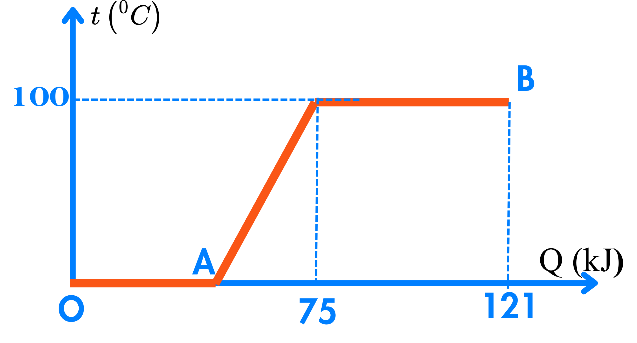
\includegraphics[width=4.5cm]{figures/fig_cau02_p2.png}
	}
	\choiceTF
	{\True Đoạn $OA$ cho biết khối lượng nước đá nhận nhiệt lượng để thực hiện quá trình nóng chảy}
	{\True Tại điểm $A$, nước đá đã hoàn toàn chuyển sang thể lỏng}
	{\True Khối nước đá ban đầu trong nhiệt lượng kế là $100\text{ g}$}
	{Kể từ lúc bắt đầu đun cho đến khi lượng nước trong bình bay hơi hết thì tổng nhiệt lượng mà nước đá nhận là $121\text{ kJ}$}
	\loigiai{
	\begin{itemchoice}
		\itemch Đoạn $OA$ nhiệt độ giữ không đổi ở $0^\circ\text{C}$ biểu thị quá trình thu nhiệt để nóng chảy hoàn toàn.		\itemch Tại điểm $A$, kết thúc quá trình nóng chảy, nước đá đã tan hoàn toàn thành nước ở $0^\circ\text{C}$.
		\itemch Từ điểm $A$ ($0^\circ\text{C}$) đến khi nhiệt độ đạt $100^\circ\text{C}$, nhiệt lượng nước nhận vào là:
		\[
		\Delta Q = Q_{75} - Q_A = mc\Delta t = m \times 4200 \times 100 = 420\,000m\text{ J} = 420m\text{ kJ}.
		\]
		Mặt khác, nhiệt lượng nóng chảy đoạn $OA$: $Q_A = m\lambda = 3{,}3 \times 10^5 m\text{ J} = 330m\text{ kJ}$.\\
		Do đó nhiệt lượng tại mốc $100^\circ\text{C}$:
		\[
		Q_{75} = Q_A + \Delta Q = 330m + 420m = 750m\text{ kJ} \Rightarrow 750m = 75 \Rightarrow m = 0{,}1\text{ kg} = 100\text{ g}.
		\]
		\itemch Nhiệt lượng cần thiết để hóa hơi hoàn toàn $100\text{ g}$ nước ở $100^\circ\text{C}$ là:
		\[
		Q_{hh} = mL = 0{,}1 \times 2{,}26 \times 10^6 = 226\,000\text{ J} = 226\text{ kJ}.
		\]
		Tổng nhiệt lượng kể từ lúc bắt đầu đun đến khi hóa hơi hết:
		\[
		Q_{tong} = 75 + 226 = 301\text{ kJ} \neq 121\text{ kJ}.
		\]
		(Mốc $121\text{ kJ}$ trên đồ thị chỉ mới hóa hơi được một phần nước).
	\end{itemchoice}
	}
\end{ex}

\vspace{0.15cm}
\begin{flushleft}
	{\color{blue!50!green}\fbox{\fontfamily{qag}\bfseries\selectfont PHẦN III. Câu trắc nghiệm trả lời ngắn (2,0 điểm)}}
	\textit{\small (Thí sinh trả lời từ câu 1 đến câu 4.)}
\end{flushleft}
\setcounter{ex}{0}

% Câu 15
\begin{ex}
	\macau{ID: VL12-HBT2526-C15}Một lượng khí bị nén bởi một công có độ lớn $150\text{ kJ}$. Khí nóng lên và tỏa ra môi trường một nhiệt lượng $95\text{ kJ}$. Độ biến thiên nội năng của khí là bao nhiêu $\text{kJ}$?

	\par\shortans[oly]{55}
	\loigiai{
		Khí nhận công nên $A = 150\text{ kJ}$.\\
		Khí truyền nhiệt cho môi trường nên $Q = -95\text{ kJ}$.\\
		Độ biến thiên nội năng của khối khí:
		\[
		\Delta U = A + Q = 150 + (-95) = 55\text{ kJ}.
		\]
	}
\end{ex}

% Câu 16
\begin{ex}
	\macau{ID: VL12-HBT2526-C16}Một nhiệt kế bị hỏng có hai nhiệt độ mốc trong thang Celsius là $-2^\circ\text{C}$ tại điểm đóng băng của nước tinh khiết và $102^\circ\text{C}$ ứng với điểm sôi của nước ở áp suất tiêu chuẩn. Một học sinh dùng nhiệt kế này để đo nhiệt độ của một chất thì đọc được giá trị là $65{,}6^\circ\text{C}$. Thực tế, nhiệt độ chính xác của chất đó là bao nhiêu $^\circ\text{C}$?

	\par\shortans[oly]{65}
	\loigiai{
		Khoảng cách nhiệt độ từ điểm đóng băng đến điểm sôi trên thang của nhiệt kế hỏng:
		\[
		102 - (-2) = 104\text{ độ chia}.
		\]
		Khoảng cách này ứng với $100^\circ\text{C}$ trên thang đo chuẩn.\\
		Giá trị đọc được là $65{,}6^\circ\text{C}$, tức là cách điểm đóng băng của nhiệt kế hỏng một khoảng:
		\[
		65{,}6 - (-2) = 67{,}6\text{ độ chia}.
		\]
		Nhiệt độ chính xác thực tế của chất đó:
		\[
		t = \dfrac{67{,}6}{104} \times 100^\circ\text{C} = 65^\circ\text{C}.
		\]
	}
\end{ex}

% Câu 17
\begin{ex}
	\macau{ID: VL12-HBT2526-C17}Một nhà máy thép mỗi lần luyện thu được $35\text{ tấn}$ thép. Biết rằng nhiệt nóng chảy riêng của thép là $2{,}77 \times 10^5\text{ J/kg}$. Nhiệt lượng mà thép cần nhận vào để nóng chảy hoàn toàn tại nhiệt độ nóng chảy trong mỗi lần luyện bằng bao nhiêu $\text{MJ}$?

	\par\shortans[oly]{9695}
	\loigiai{
		Khối lượng thép mỗi lần luyện: $m = 35\text{ tấn} = 35\,000\text{ kg}$.\\
		Nhiệt lượng cần cung cấp để làm nóng chảy hoàn toàn lượng thép tại nhiệt độ nóng chảy:
		\[
		Q = m \lambda = 35\,000 \times 2{,}77 \times 10^5 = 9\,695 \times 10^6\text{ J} = 9695\text{ MJ}.
		\]
	}
\end{ex}

% Câu 18
\begin{ex}
	\macau{ID: VL12-HBT2526-C18}Biết nhiệt độ sôi của rượu là $78^\circ\text{C}$. Một lượng rượu đang trong quá trình hóa hơi ở nhiệt độ sôi thì nhiệt độ của lượng hơi đó trong quá trình hóa hơi là bao nhiêu $^\circ\text{C}$?

	\par\shortans[oly]{78}
	\loigiai{
		Trong suốt quá trình hóa hơi ở nhiệt độ sôi, nhiệt độ của chất lỏng và hơi luôn không đổi và bằng nhiệt độ sôi của chất đó. Do đó nhiệt độ của lượng hơi là $78^\circ\text{C}$.
	}
\end{ex}

\vspace{0.15cm}
\begin{flushleft}
	{\color{blue!50!green}\fbox{\fontfamily{qag}\bfseries\selectfont PHẦN IV. Tự luận (3,0 điểm)}}
	\textit{\small (Thí sinh trình bày lời giải chi tiết cho các câu hỏi sau.)}
\end{flushleft}
\setcounter{ex}{0}

% Câu 19
\begin{ex}
	\macau{ID: VL12-HBT2526-C19}\textbf{(1,0 điểm)} Một vật bằng nhôm khối lượng $0{,}5\text{ kg}$ được làm lạnh từ $100^\circ\text{C}$ xuống $20^\circ\text{C}$. Biết nhiệt dung riêng của nhôm $c = 880\text{ J/(kg}\cdot\text{K)}$.
	\begin{enumerate}[a)]
		\item Tính độ biến thiên nội năng của vật.
		\item Nội năng của vật tăng hay giảm? Giải thích vì sao?
	\end{enumerate}
	\loigiai{
	\begin{enumerate}[a)]
		\item Nhiệt lượng mà vật bằng nhôm tỏa ra môi trường:
		\[
		Q = m c (t_2 - t_1) = 0{,}5 \times 880 \times (20 - 100) = -35\,200\text{ J}.
		\]
		Vì vật chỉ truyền nhiệt lượng mà không thực hiện công ($A = 0$), theo định luật I nhiệt động lực học:
		\[
		\Delta U = Q = -35\,200\text{ J}.
		\]
		Độ lớn biến thiên nội năng của vật là $35\,200\text{ J}$.
		\item Nội năng của vật \textbf{giảm} vì:
		\begin{itemize}
			\item Nhiệt độ của vật giảm từ $100^\circ\text{C}$ xuống $20^\circ\text{C}$, làm cho động năng chuyển động nhiệt của các phân tử cấu tạo nên vật giảm, dẫn đến nội năng của vật giảm.
			\item Đồng thời vật tỏa nhiệt ra môi trường xung quanh ($Q < 0 \Rightarrow \Delta U < 0$).
		\end{itemize}
	\end{enumerate}
	}
\end{ex}

% Câu 20
\begin{ex}
	\macau{ID: VL12-HBT2526-C20}\textbf{(2,0 điểm)} Người ta đổ $1\text{ kg}$ nước ở nhiệt độ $20^\circ\text{C}$ vào một ấm điện có công suất $2200\text{ W}$ để đun (bỏ qua mọi hao phí nhiệt lượng và nhiệt dung của ấm). Biết nhiệt dung riêng của nước là $4200\text{ J/(kg}\cdot\text{K)}$.
	\begin{enumerate}[a)]
		\item Tính thời gian kể từ lúc bắt đầu đun đến khi nước trong ấm sôi.
		\item Ngay khi nước sôi người ta đổ thêm $0{,}5\text{ kg}$ nước (cùng bản chất với nước trong ấm) ở nhiệt độ $30^\circ\text{C}$ vào ấm. Hỏi sau bao lâu kể từ lúc đổ thêm nước thì nước trong ấm lại sôi?
	\end{enumerate}
	\loigiai{
	\begin{enumerate}[a)]
		\item Nhiệt lượng cần cung cấp để đun sôi $1\text{ kg}$ nước từ $20^\circ\text{C}$ lên $100^\circ\text{C}$:
		\[
		Q_1 = m_1 c (t_s - t_1) = 1 \times 4200 \times (100 - 20) = 336\,000\text{ J}.
		\]
		Vì bỏ qua hao phí nhiệt nên công suất tỏa nhiệt của ấm bằng công suất có ích:
		\[
		P \cdot t_1 = Q_1 \Rightarrow t_1 = \dfrac{Q_1}{P} = \dfrac{336\,000}{2200} \approx 152{,}73\text{ s} \approx 2\text{ phút } 33\text{ giây}.
		\]
		\item Ngay khi nước sôi, trong ấm có $1\text{ kg}$ nước ở $100^\circ\text{C}$. Đổ thêm $0{,}5\text{ kg}$ nước ở $30^\circ\text{C}$ vào.\\
		Để toàn bộ lượng nước trong ấm sôi lại ở $100^\circ\text{C}$, theo định luật bảo toàn năng lượng, tổng nhiệt lượng mà ấm điện cần cung cấp chính là nhiệt lượng cần thiết để nâng $0{,}5\text{ kg}$ nước vừa đổ vào từ $30^\circ\text{C}$ lên $100^\circ\text{C}$:
		\[
		Q_2 = m_2 c (t_s - t_2) = 0{,}5 \times 4200 \times (100 - 30) = 147\,000\text{ J}.
		\]
		Thời gian cần thiết để nước trong ấm sôi lại:
		\[
		t_2 = \dfrac{Q_2}{P} = \dfrac{147\,000}{2200} \approx 66{,}82\text{ s} \approx 1\text{ phút } 7\text{ giây}.
		\]
	\end{enumerate}
	}
\end{ex}
